\documentclass[12pt,letterpaper]{article}

\usepackage[utf8]{inputenc}
\usepackage[T1]{fontenc}
\usepackage{amsmath}
\usepackage{amsfonts}
\usepackage{amssymb}
\usepackage{amsthm}
\usepackage[left=2cm,right=2cm,top=2cm,bottom=2cm,headheight=22pt]{geometry}
\usepackage{fancyhdr}
\usepackage{setspace}
\usepackage{lastpage}
\usepackage{graphicx}
\usepackage{caption}
\usepackage{subcaption}
\usepackage{wrapfig}
\usepackage{paralist}
\usepackage{url}
\usepackage{tikz}

\theoremstyle{definition}
\newtheorem{question}{Question}
\newtheorem{example}{Example}
\newtheorem{exercise}[question]{Exercise}
\newtheorem*{challenge}{Challenge}

\begin{document}

%Paramètres de mise en forme des paragraphes selon les normes françaises
\setlength{\parskip}{1ex plus 0.5ex minus 0.2ex}
\setlength{\parindent}{0pt}

%Paramètres relatifs aux en-têtes et pieds de page.
\pagestyle{fancy}
\lhead{Theron J Hitchman}
\chead{\Large Reading and Guided Practice \#8}
\rhead{Fall 2013}
\lfoot{\emph{Math and Decision Making}}
\cfoot{}
\rfoot{\emph{\thepage\ of \pageref{LastPage}}}

\section*{Introduction}
We introduce the notion of \emph{tricolorability} for planar projection diagrams of knots and links. 
We explore some examples and learn how to test a diagram.

\section*{Goals}
At the end of this assignment, a student should be able to:
\begin{compactitem}
\item Determine if a given planar projection diagram of a knot or link is or is not tricolorable.
\end{compactitem}
A student might also be able to:
\begin{compactitem}
\item Solve a challenging problem about tricolorability.
\end{compactitem}

\section*{Reading and Questions for 16 September}

Suppose you have a planar projection diagram for a knot or a link and three bright, shiny new crayons.
(Knot theorists typically use red, green, and blue.)
%Can you color the lines of your diagram with these three colors?
%Of course you can! 
%Put the colors wherever you like. 
%To make things more interesting, we will impose some rules.
The big question will be, \emph{can you color the diagram while following some strange-sounding rules}?
For now, consider this a little game.
Later, we will see how it is important for the theory of knots and links.

\subsection*{Tricolorability}

First, we need the idea of a \emph{strand} of planar projection of a knot or link.
A \emph{strand} is one piece of the planar projection from one undercrossing to another with only overcrossings in between.
For example, the standard unknot has one strand, and the standard trefoil has three strands.
Note that at any crossing, we will have \textbf{three} strands coming together, the two understrands and the one overstrand.

\begin{figure}[h!]
    \centering
    \begin{subfigure}{.3\textwidth}
        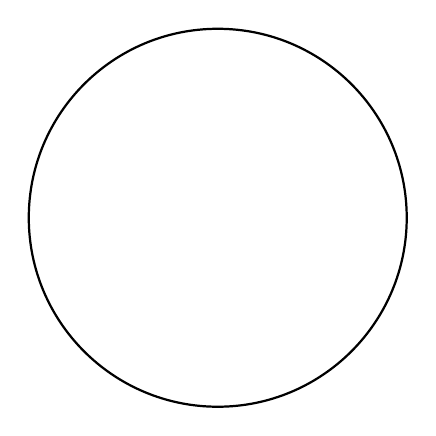
\begin{tikzpicture}[scale=1,cap=round,>=latex]
            \draw[thick] (0cm,0cm) circle(2.4cm);
        \end{tikzpicture}
        \caption{The Unknot}
    \end{subfigure}
    \hspace{1cm}
    \begin{subfigure}{.3\textwidth}
        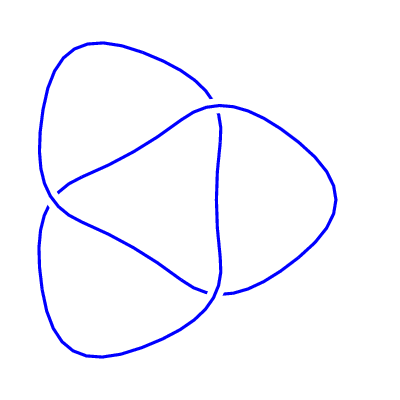
\includegraphics[width=\textwidth]{knotpics/3_1mirror.png}
        \caption{A Trefoil}
    \end{subfigure}
    \caption{Two of our simplest examples.}
\end{figure}

\begin{exercise}
Indentify the strands of the unknot and the trefoil in the pictures above.
\end{exercise}

We shall say that a planar projection diagram is \emph{tricolorable} if each strand of the knot or link can be given one of three colors (it helps to think of them as red, blue, and green), subject to the following two rules:
\begin{compactitem}
\item At each crossing, either the three strands all have the same color, or they are all different colors.
\item At least two colors get used in the process.
\end{compactitem}

\begin{exercise}
Show that the trefoil knot is tricolorable by choosing colors for the standard planar projection.
\end{exercise}

(If it feels unfamiliar to you, the word \emph{show} as instructions for an exercise means come up with an argument explaining why the statement made is true.)

\begin{exercise}
Show that the unknot is not tricolorable by noting that one of the conditions is impossible for a standard circle projection.
\end{exercise}

\begin{exercise}
Show that the ``unlink with two components'' is tricolorable.
(This is the link with two circles, which happen to not interact at all.
It is just two circles side-by-side.)
\end{exercise}

\begin{figure}[h]
    \centering
    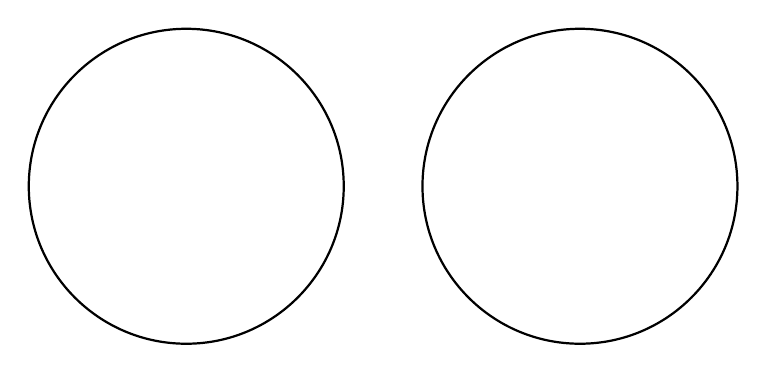
\begin{tikzpicture}[scale=1,cap=round,>=latex]
        \draw[thick] (0cm,0cm) circle(2cm);
        \draw[thick] (5cm,0cm) circle(2cm);
    \end{tikzpicture}
    \caption{The Unlink with Two Components}
\end{figure}

\section*{Examples in Detail}
Let us consider some more complicated examples. 
Below are some planar projection diagrams of knots with 5 and 8 crossings, respectively.

\begin{figure}[h]
    \centering
    \begin{subfigure}{.25\textwidth}
        \centering
        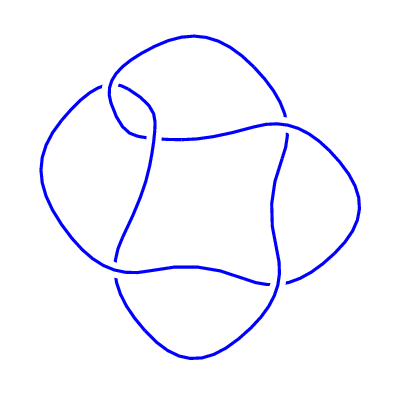
\includegraphics[width=\textwidth]{knotpics/5_2.png}
    \end{subfigure}
    \hspace{1cm}
    \begin{subfigure}{.25\textwidth}
        \centering
        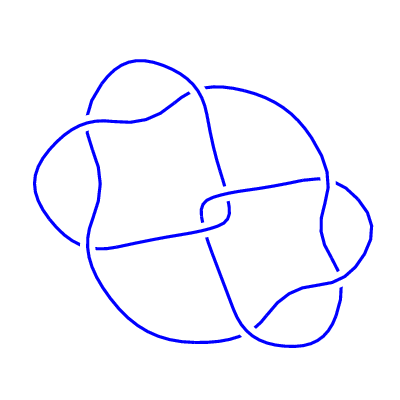
\includegraphics[width=\textwidth]{knotpics/8_5.png}
    \end{subfigure}
    \caption{Two interesting planar projections.}
\end{figure}


\subsection*{Showing a projection is not tricolorable}

\begin{wrapfigure}{l}{.5\textwidth}
    \centering
    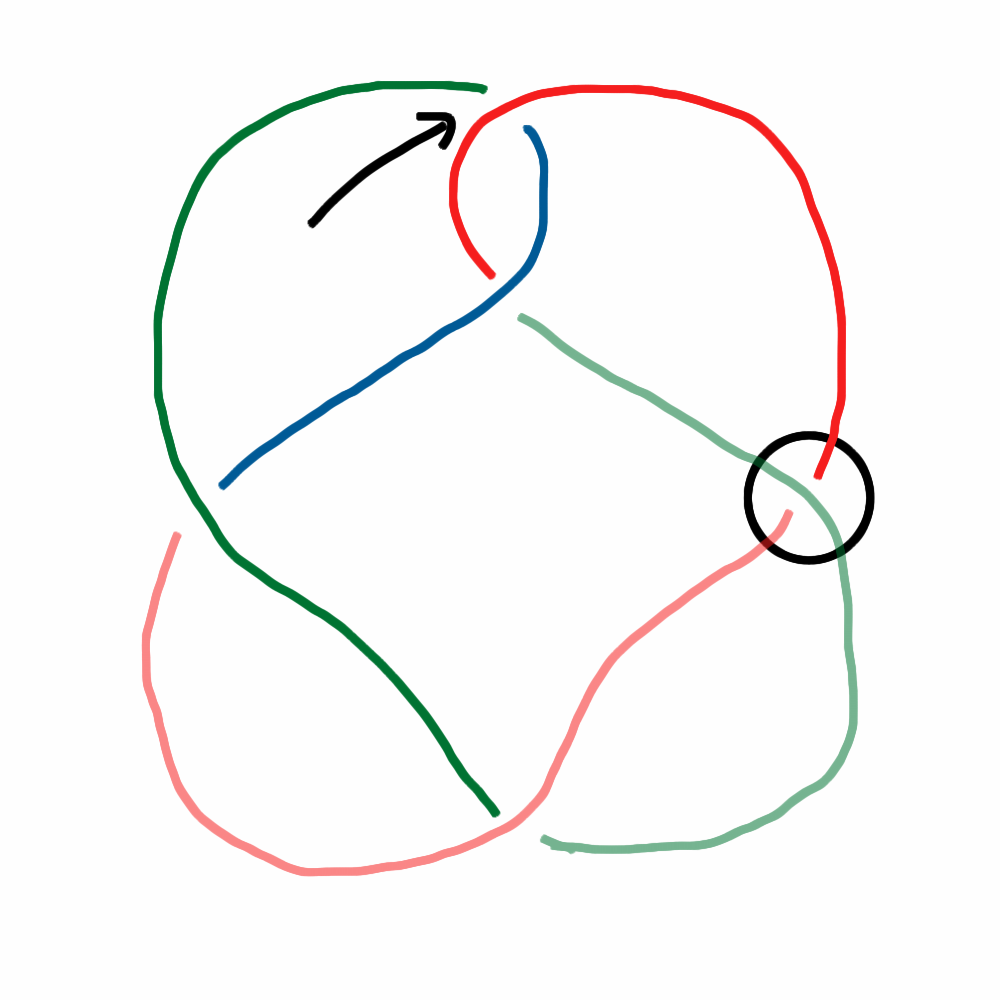
\includegraphics[width=.3\textwidth]{knotpics/nocolor1.png}
\end{wrapfigure}
The projection with five crossings is not tricolorable.
Here is how you can see this. 
We begin at the top crossing indicated by the arrow. 
By the first rule, either this crossing has all three colors at it, or none.
Let us begin by assuming that this crossing has all three colors.
We shall choose them as shown in the diagram at left.


Where the original blue and green strands come back together, the third strand must be red, by the first rule.
Similarly, where the original red and blue strands come back together, the third strand must be green.
This creates a problem at the crossing indicated in the diagram.
There are now two green strands and one red strand at this crossing, which violates our first rule. We conclude that the top crossing cannot have three different colors at it.

\begin{wrapfigure}{r}{.5\textwidth}
    \centering
    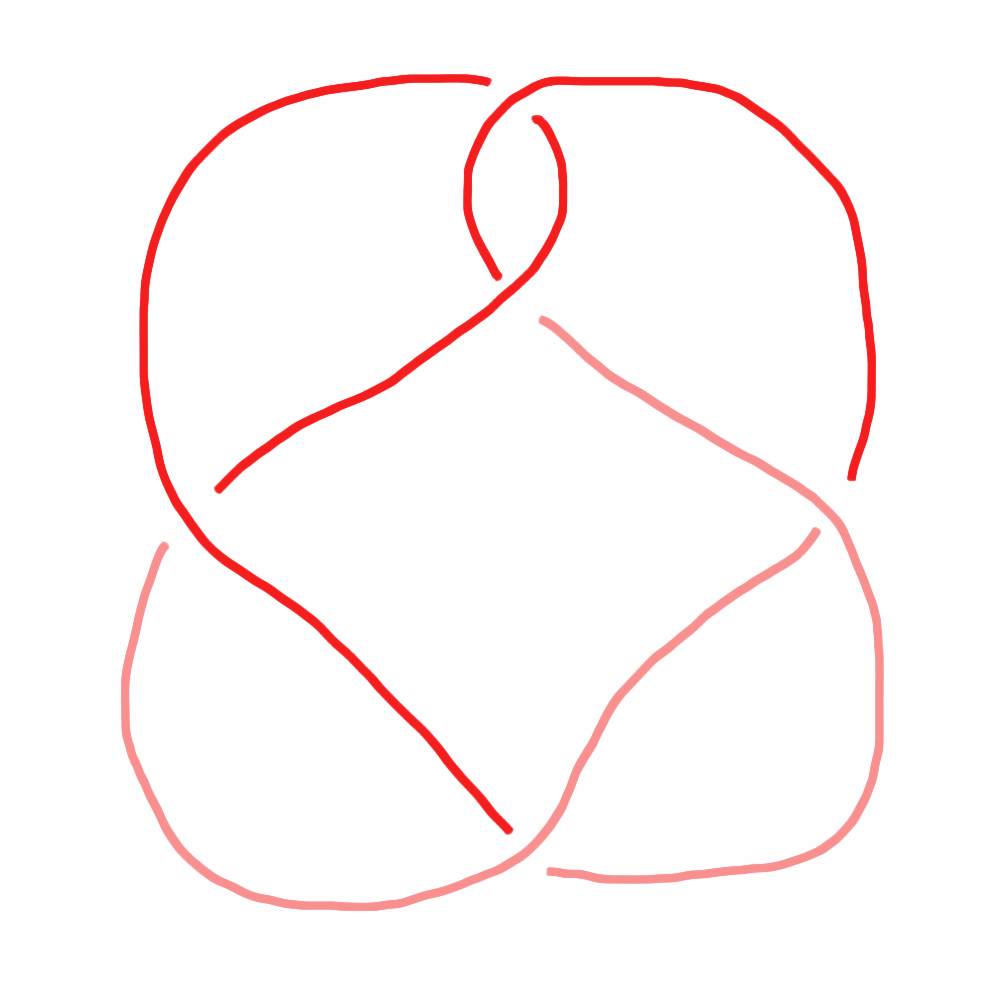
\includegraphics[width=.3\textwidth]{knotpics/nocolor2.png}
\end{wrapfigure}
The only way to proceed then is to have a top crossing with only one color at it.
Let us choose red.
Where two strands that are already red come together at a crossing, the third strand must also be red.
We use this reasoning at the two new strands, and find that if the top crossing is all red, then the whole diagram must be red. 
This contradicts our second rule. 
Therefore, the top crossing cannot be only one color.

Since our top crossing cannot have all three colors, and it cannot have only one color, we deduce that this projection is not tricolorable.

\subsection*{Showing a projection is tricolorable}

\begin{wrapfigure}{l}{.5\textwidth}
    \centering
    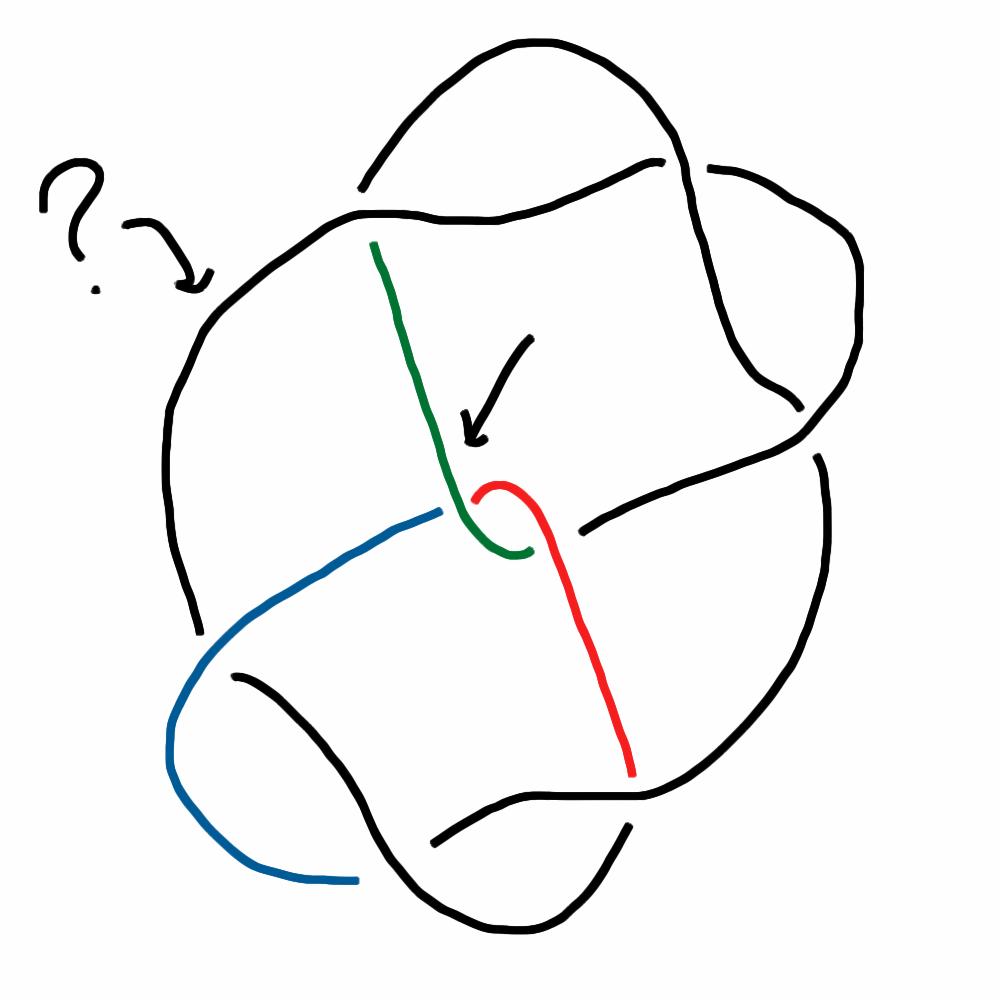
\includegraphics[width=.3\textwidth]{knotpics/colorable1.png}
\end{wrapfigure}
The example with 8 crossings is tricolorable.
Let us begin with the middle crossing indicated by the arrow.
We assume that this crossing has three colors at it, and choose an arrangment of colors for the strands involved.
Note that the strand on the far right is not determined, yet.
We must check through the possibilities: It is either red, green, or blue. 
One at a time, we try these out and see what the first rule forces on us.
But if we choose blue, red, or green we find somewhere else a crossing which contradicts rule one.
(One such crossing is circled in each diagram.)
\begin{figure}
    \centering
    \begin{subfigure}{.3\textwidth}
        \centering
        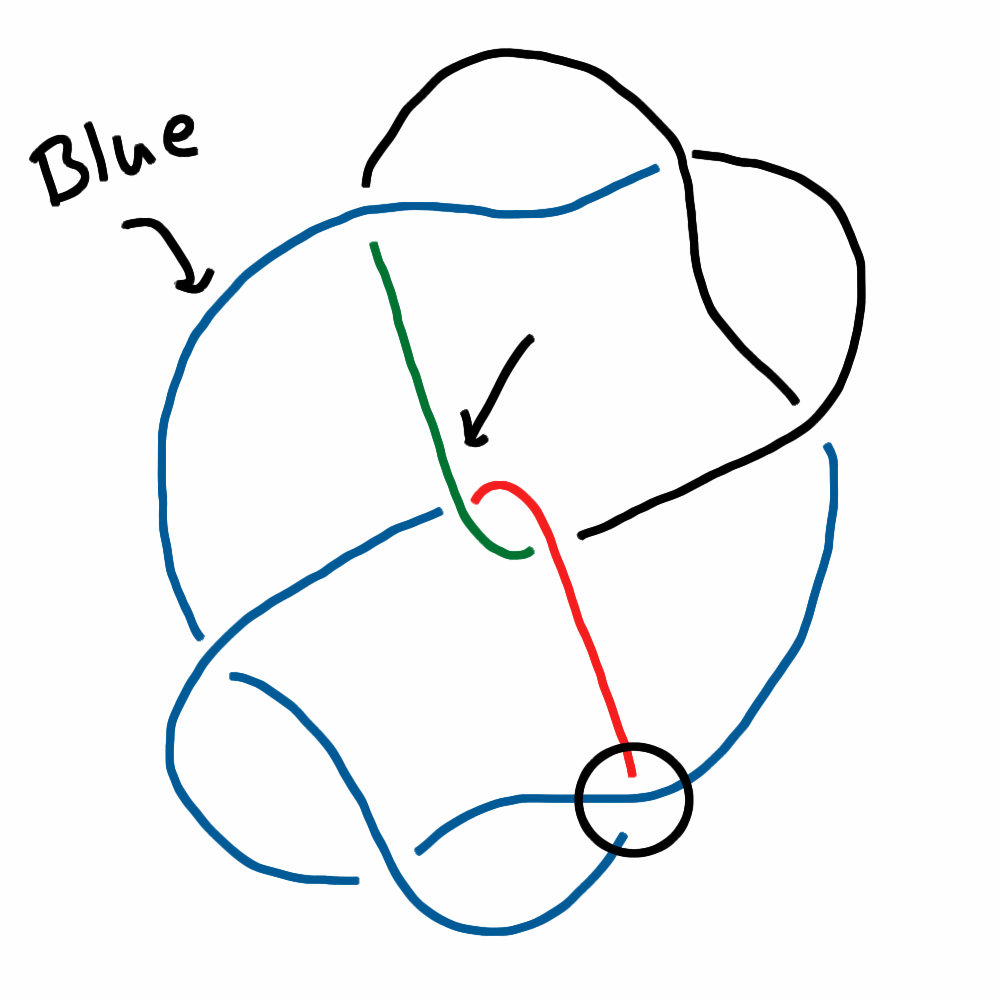
\includegraphics[width=\textwidth]{knotpics/colorable2.png}
        \caption{Trying blue.}
    \end{subfigure}
    \quad
    \begin{subfigure}{.3\textwidth}
        \centering
        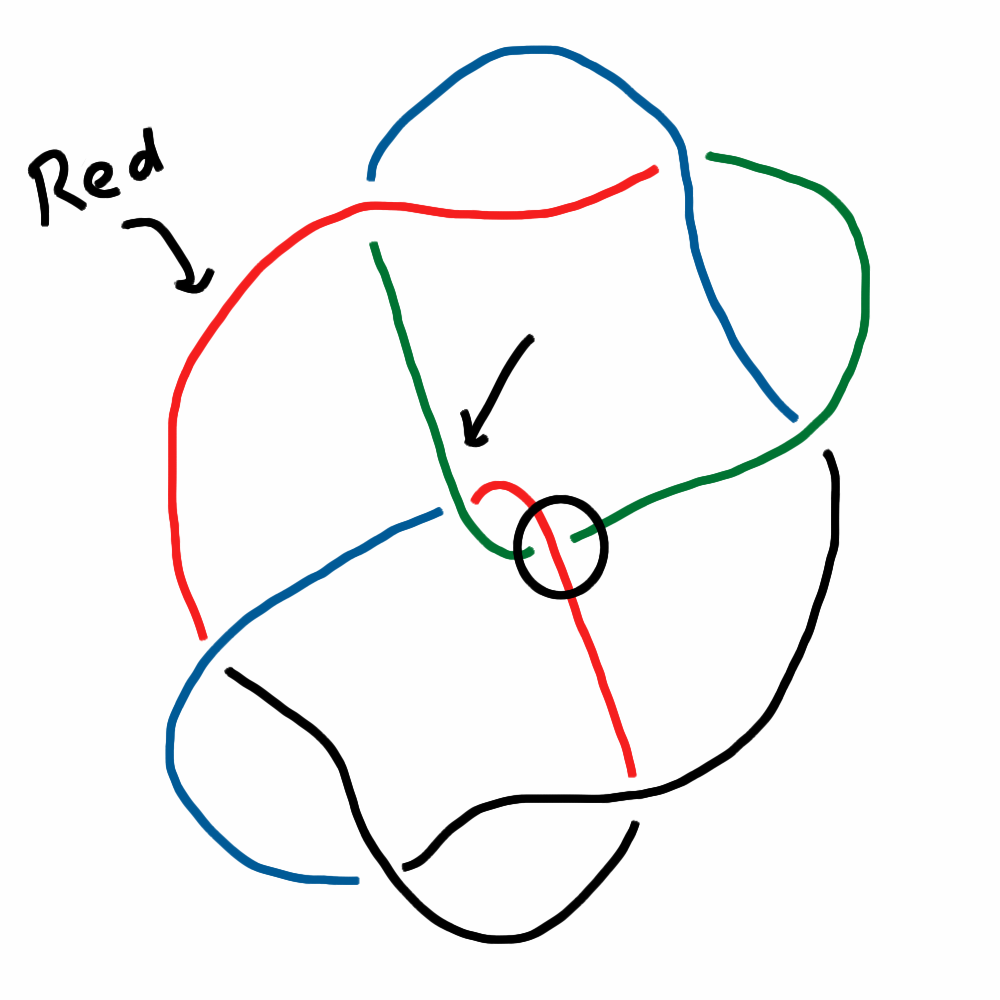
\includegraphics[width=\textwidth]{knotpics/colorable3.png}
        \caption{Trying red.}
    \end{subfigure}
    \quad
    \begin{subfigure}{.3\textwidth}
        \centering
        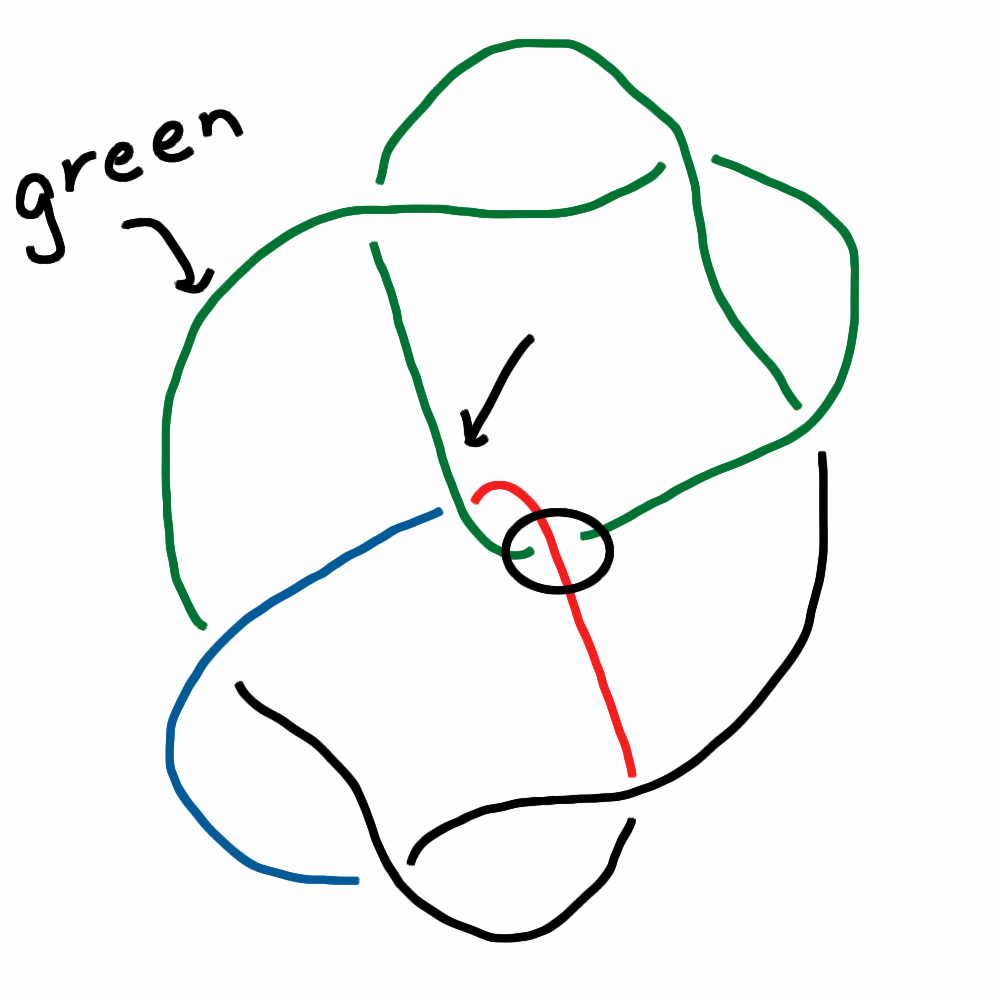
\includegraphics[width=\textwidth]{knotpics/colorable4.png}
        \caption{Trying green.}
    \end{subfigure}
    \caption{Working out a coloring for our projection diagram.}
\end{figure}

Since none of these work, this interior crossing where we started must have only one color at it.
We try one more time using green as our starting color.
This time, we choose the far left-hand strand to be red, and see what ends up determined by repeated application of the first rule. 
Following along, we get this.
\begin{figure}[h]
    \centering
    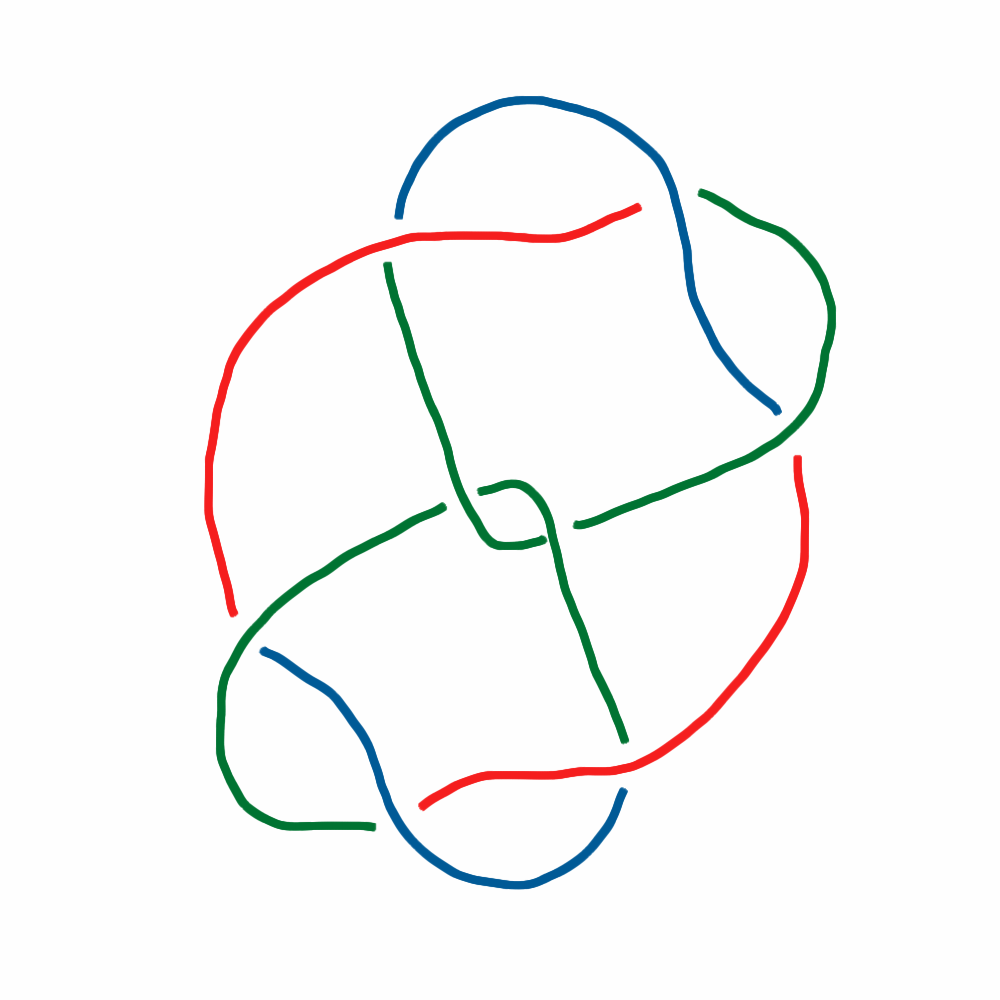
\includegraphics[width=.5\textwidth]{knotpics/colorable5.png}
    \caption{A tricoloring of this planar projection diagram.}
\end{figure}

Note that this is consistent with the rules at all of the crossings!
(It is a good idea to go back and check all of the crossings when you are done.)

And that is it.
Since we have found an arrangment of colors which satisfies the rules, this planar projection diagram is tricolorable.


\subsection*{Practice}

\begin{exercise}
Decide which of these three knots with six crossings are tricolorable.
\end{exercise}

\begin{figure}[h]
    \centering
    \begin{subfigure}{.3\textwidth}
        \centering
        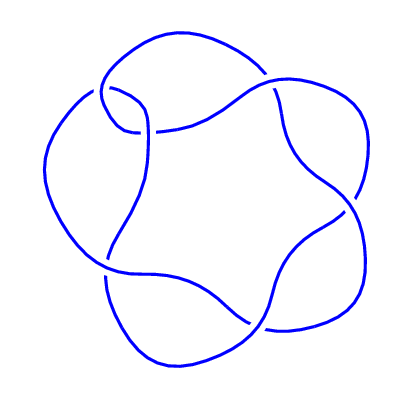
\includegraphics[width=\textwidth]{knotpics/6_1.png}
        \caption{A projection of knot $6_1$.}
    \end{subfigure}
    \quad
    \begin{subfigure}{.3\textwidth}
        \centering
        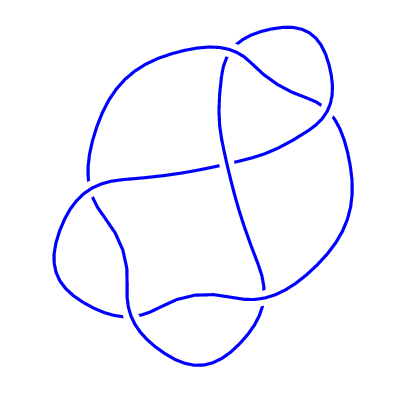
\includegraphics[width=\textwidth]{knotpics/6_2.png}
        \caption{A projection of knot $6_2$.}
    \end{subfigure}
    \quad
    \begin{subfigure}{.3\textwidth}
        \centering
        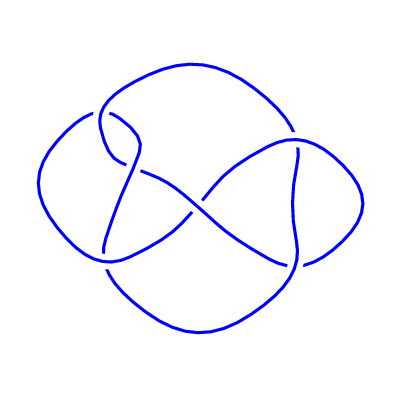
\includegraphics[width=\textwidth]{knotpics/6_3.png}
        \caption{A projection of knot $6_3$.}
    \end{subfigure}
\caption{Three planar projections with 6 crossings.}
\end{figure}


\begin{thebibliography}{9}

\bibitem{Adams}
	Colin C. Adams,
	\emph{The Knot Book},
	American Mathematical Society,
	2004.

\bibitem{knotinfo}
	J. C. Cha and C. Livingston,
	KnotInfo: Table of Knot Invariants,
	\url{http://www.indiana.edu/~knotinfo},
	accessed: September 6, 2013.


\end{thebibliography}

\end{document}
%sagemathcloud={"zoom_width":100}